% Chapter Template

\chapter{Examples} % Main chapter title

\label{sec:Examples} % Change X to a consecutive number; for referencing this chapter elsewhere, use \ref{ChapterX}


In this chapter, I will go through some examples, illustrating how to use the code base to learn and solve various puzzles. For each section, simple examples of code will be indicated in air force blue \afblue \textbf{python code} \black paragraphs, and can easily be run from command line or copied into a script and run from your favourite IDE.


%-----------------------------------
%	SECTION 1
%-----------------------------------
\section{Learners}


%-----------------------------------
%	SUBSECTION 1.1
%-----------------------------------
\subsection{Perfect Learner}
\label{PLSS}


%-----------------------------------
%	SUBSECTION 1.2
%-----------------------------------
\subsection{Deep Learner}
\label{DLSS}
blabla

%-----------------------------------
%	SUBSECTION 1.3
%-----------------------------------
\subsection{Deep Reinforcement Learner}
\label{DRLSS}

blabla

%-----------------------------------
%	SECTION 2
%-----------------------------------

\section{Solvers}

%-----------------------------------
%	SUBSECTION 2.1
%-----------------------------------
\subsection{Blind search}
%-----------------------------------
%	SUBSECTION 2.1.1
%-----------------------------------
\subsubsection{BFS}
\label{BFSSS}
%-----------------------------------
%	SUBSECTION 2.1.2
%-----------------------------------
\subsubsection{DFS}
\label{DFSSS}



%-----------------------------------
%	SUBSECTION 2.2
%-----------------------------------
\subsection{Naive Sliding Puzzle Solver}
As a comparison point for other sliding puzzle solvers, I have implemented a naive sliding puzzle solver, which does what most beginner players would intuitively do when solving the sliding puzzle by hand: solve the top row, then the left column, and keep iterating until done. Notice that once either the top row or left column is solved, there is no longer any need to modify it, we have simply reduced the problem to a sub-problem of reduced dimension. For the interested reader, the details of the algorithm are as follows:
\begin{itemize}
\item if n and m are both equal to 2, we just keep moving the empty tile clock-wise until the puzzle is solved. Notice that this is bound to work, since moving clock-wise or counter-clock-wise are the two ony possible moves, and one of them is just un-doing the other one, therefore the only possible sequence of move in a (n=2, m=2) puzzle is to either keep moving clock-wise or counter-clock-wise.
\item if n $\geq$ m, we solve the top row
\item otherwise we solve the left column
\end{itemize}
Solving the top row of a n by m puzzle (left column is similar, mutatis mutandis, so I will not detail it) is accomplished as follows:
\\
\textbf{naive algorithm - top-row solver}
\begin{enumerate}
\item \label{s1} we sort the tiles (which since we are potentially dealing with a sub-problem, are not necessarily 1 to $m* n - 1$), and select the m smaller ones $t_{1}, ..., t_{m-1}, t_{m}$.
\item \label{s2} we place $t_{m}$ in the bottom-left corner
\item \label{s3} we place $t_{1}, ..., t_{m-2}$ to their respective positions (in that order, and making sure not to undo any previous steps as we do so)
\item \label{s4} we place $t_{m-1}$ in the top-right corner
\item \label{s5} we then move $t_{m}$ just under $t_{m-1}$
\item \label{s6} we move the empty tile to the left of $t_{m-1}$
\item \label{s7} finally we move the empty tile right and then down to put $t_{m-1}$ and $t_{m}$ in place.
\end{enumerate}
In order to move the tiles, we have written a few simple routines which can move the empty tile from its current position next to (above, below, left or right) any tile, and then can move that tile to another position, all the while avoiding to go through previously moved tiles (hence the particular order in which we move the different tiles above). The only case where the above algorithm can get stuck is when both n and m are equal to 3 and that by step \ref{s6} we end up with $t_{3}$ under the empty tile. We have handcrafted a sequence of moves to solve this particular position. Other than this one particular case, the above naive algorithm is guaranteed to succeed (and is obviously quite fast in terms of run time, though not elegant).
\\
\\
As a concrete example, let us assume we started with the following (n=6, m=6) puzzle:
\\
\begin{thityfive}
\setrow{6}{14,27,6,  2,5,18}
\setrow{5}{21,29,13,23,35,30}
\setrow{4}{26,3,7,9,24,19}
\setrow{3}{22,12,11,17,16,33}
\setrow{2}{32,10,20,25,34,28}
\setrow{1}{8,4,15,31, ,1}
\end{thityfive}
\\
\\
After one call to solve the top row and the left column, we are left with solving the (n=5,m=5) sub-puzzle in blue:
\\
\begin{thityfive}
\setrow{6}{1,2,3,4,5,6}
\setrow{5}{7,\blue9,\blue17,\blue27,\blue18,\blue35}
\setrow{4}{8,\blue23,\blue11,\blue15,\blue24,\blue21}
\setrow{3}{9,\blue20,\blue8,\blue29,\blue33,\blue10}
\setrow{2}{10,\blue22,\blue30,\blue14,\blue32,\blue16}
\setrow{1}{11,\blue ,\blue12,\blue26,\blue34,\blue28}
\end{thityfive}
\\
\\
Let us now detail how the \textbf{naive algorithm} will solve the top row if that sub-puzzle:
\\
\begin{twentyfour}
\setrow{5}{9,17,27,18,35}
\setrow{4}{23,11,15,24,21}
\setrow{3}{20,8,29,33,10}
\setrow{2}{22,30,14,32,16}
\setrow{1}{ ,12,26,34,28}
\end{twentyfour}
\\
\\
step \ref{s1} above will decide to solve the top row by placing $t_{1}, ..., t_{5}$ = $\blue 8, 9, 10, 11, 12$ in that order as the top row. Steps \ref{s2} to \ref{s7} will yield in order:
\\
\begin{twentyfour}
\setrow{5}{\blue9,17,27,18,35}
\setrow{4}{23,\blue11,15,24,21}
\setrow{3}{20,\blue8,29,33,\blue10}
\setrow{2}{22,30,14,32,16}
\setrow{1}{ ,\blue12,26,34,28}
\end{twentyfour}
%
\begin{twentyfour}
\setrow{5}{\blue9,17,27,18,35}
\setrow{4}{23,\blue11,15,24,21}
\setrow{3}{20,\blue8,29,33,\blue10}
\setrow{2}{22,30,14,32,16}
\setrow{1}{\color{red}12\color{red}, ,26,34,28}
\end{twentyfour}
%
\begin{twentyfour}
\setrow{5}{\red 8,\red 9,\red 10,,18}
\setrow{4}{17,15,27,24,35}
\setrow{3}{\blue11,23,29,21,33}
\setrow{2}{20,22,14,32,16}
\setrow{1}{\red 12,30,26,34,28}
\end{twentyfour}
\\
\begin{twentyfour}
\setrow{5}{\red 8, \red 9, \red 10,,\red 11}
\setrow{4}{23,29,21,18,24}
\setrow{3}{17,15,27,33,35}
\setrow{2}{20,22,14,32,16}
\setrow{1}{\red 12,30,26,34,28}
\end{twentyfour}
%
\begin{twentyfour}
\setrow{5}{\red 8,\red 9,\red 10,18,\red 11}
\setrow{4}{29,27,32, ,\red 12}
\setrow{3}{23,21,33,35,24}
\setrow{2}{15,17,22,14,16}
\setrow{1}{30,20,26,34,28}
\end{twentyfour}
%
\begin{twentyfour}
\setrow{5}{\red 8, \red 9, \red 10, \red 11, \red 12}
\setrow{4}{29,27,32,18, }
\setrow{3}{23,21,33,35,24}
\setrow{2}{15,17,22,14,16}
\setrow{1}{30,20,26,34,28}
\end{twentyfour}
\\
\\
and we are left with solving the bottom sub-puzzle (n=4,m=5):
\\
\begin{twenty}
\setrow{4}{29,27,32,18, }
\setrow{3}{23,21,33,35,24}
\setrow{2}{15,17,22,14,16}
\setrow{1}{30,20,26,34,28}
\end{twenty}

\afblue
\paragraph{}{\textbf{python code -- naive solver}}
\begin{python}
################################################
from math import inf
from rubiks.puzzle.puzzle import Puzzle
from rubiks.solvers.solver import Solver
################################################
action_type=Solver.do_solve
n=2
puzzle_type=Puzzle.sliding_puzzle
solver_type=Solver.naive
nb_shuffles=inf
################################################
print(Solver.factory(**globals()).action())
################################################
\end{python}
\black

\begin{figure}[H]
\centering
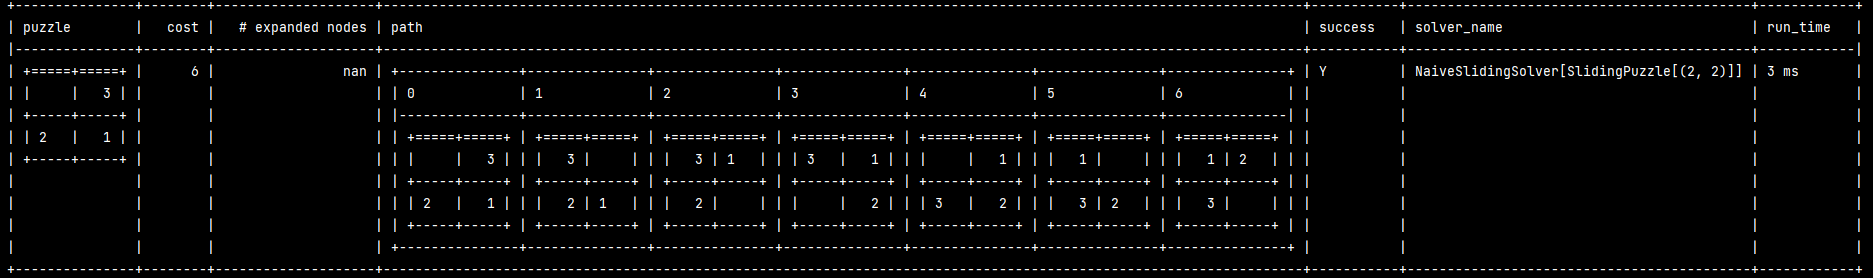
\includegraphics[scale=0.39]{./Figures/examplenaivesolver}
%\decoRule
\caption[Examples]{naive solver}
\label{fig:examplenaivesolver}
\end{figure}



%-----------------------------------
%	SUBSECTION 2.3
%-----------------------------------
\subsection{Kociemba}
TBD


%-----------------------------------
%	SUBSECTION 2.4
%-----------------------------------
\subsection{A*}
\label{ASSS}

\textbf{manhattan heuristic}

\textbf{perfect heuristic}

\textbf{deep learning heuristic}

\textbf{deep reinforcement learning heuristic}


